% SPDX-License-Identifier: CC-BY-SA-4.0
%
% Copyright (c) 2020 Philipp Le
%
% Except where otherwise noted, this work is licensed under a
% Creative Commons Attribution-ShareAlike 4.0 License.
%
% Please find the full copy of the licence at:
% https://creativecommons.org/licenses/by-sa/4.0/legalcode

\chapter{Modulation}

\begin{refsection}
	
The task of a communication system is transmitting information.

Example: Voice transmission
\begin{itemize}
	\item Voice has a spectrum from about \SI{20}{Hz} to \SI{20}{kHz}
	\item It is not feasible to transmit the spectrum directly as electromagnetic waves.
	\item The electromagnetic spectrum must be shared with myriads of other users.
	\item So, the voice is shifted to a higher frequency, for example, \SI{144.3}{MHz}.
	\item The voice is \emph{modulated} on this \emph{carrier} of \SI{144.3}{MHz}.
	\item The voice is then located from about \SI{144.28}{MHz} to \SI{144.32}{MHz}.
\end{itemize}

\begin{definition}{Modulation}
	\index{modulation} \textbf{Modulation} is the process of altering a signal -- the \index{carrier} \textbf{carrier} -- so that it contains the information of the \index{baseband} \textbf{baseband} signal.
\end{definition}

In the previous example, the voice was the baseband signal. This can be transferred to any kind of information. In this chapter, we will discuss techniques to modulate data on carriers which can be transmitted over wired and wireless channels.

\todo{Block diagram modulator}

\section{Modulation in The Time and Frequency Domain}

Generally, the carrier is a \emph{monochromatic} signal, i.e., it is a sinusoidal function. A sinusoidal function has three parameters: (angular) frequency $\omega_C$, phase $\varphi_C$ and amplitude $\hat{X}_C$.
\begin{equation}
	x_C(t) = \hat{X}_C \cos\left(\omega_C t + \varphi_C\right)
	\label{eq:ch05:carrier_timedomain}
\end{equation}
The frequency is fixed to the carrier frequency. The other two parameters can be altered and the information can be modulated into them.

There are two classes of modulation:
\begin{itemize}
	\item \textbf{Amplitude modulation} The amplitude of the carrier is altered.
	\begin{equation}
		x_{S,AM}(t) = f_{\hat{X}}(t) \cos\left(\omega_C t + \varphi_C\right)
	\end{equation}
	\item \textbf{Phase modulation} The phase of the carrier is altered.
	\begin{equation}
		x_{S,PM}(t) = \hat{X}_C \cos\left(\omega_C t + f_{\varphi}(t)\right)
	\end{equation}
\end{itemize}

\subsection{Amplitude Modulation}

\index{amplitude modulation} \textbf{\ac{AM}} is the alteration of the carrier's amplitude.

\begin{attention}
	By now, all signals are real, because the technical realization is considered. Physical signals must always be real.
\end{attention}

The carrier is a mono-chromatic signal:
\begin{equation}
	x_C(t) = \hat{X}_C \cdot \cos\left(2\pi f_C + \varphi_C\right)
\end{equation}
where
\begin{itemize}
	\item $\hat{X}_C$ is the amplitude of the carrier,
	\item $f_C$ is the carrier frequency ($2\pi f_C = \omega_C$ is carrier angular frequency), and
	\item $\varphi_C$ is the phase offset of the carrier.
\end{itemize}

The carrier amplitude can be altered by multiplying it with the instantaneous value of the baseband signal $x_B(t)$:
\begin{equation}
	x_M(t) = x_B(t) \cdot \left(1 + \mu x_C(t)\right)
	\label{eq:ch05:amdsb_timedomain}
\end{equation}
\begin{itemize}
	\item The waveform of the carrier is retained. The carrier is still present in the modulated signal. This is represented by the $+1$ in the sum.
	\item Its amplitude is changed by the instantaneous value of the baseband signal. The contribution of the baseband signal is defined by the factor $\mu$.
\end{itemize}

\begin{figure}[H]
	\centering
	
	\subfloat[Carier and signal signals]{
		\centering
		\begin{tikzpicture}
			\begin{axis}[
				height={0.15\textheight},
				width=0.6\linewidth,
				scale only axis,
				xlabel={$t$},
				ylabel={$x(t)$},
				%grid style={line width=.6pt, color=lightgray},
				%grid=both,
				grid=none,
				legend pos=outer north east,
				axis y line=middle,
				axis x line=middle,
				every axis x label/.style={
					at={(ticklabel* cs:1.05)},
					anchor=north,
				},
				every axis y label/.style={
					at={(ticklabel* cs:1.05)},
					anchor=east,
				},
				xmin=-0.5,
				xmax=8.5,
				ymin=-1.2,
				ymax=1.2,
				%xtick={0,0.125,...,1},
				%xticklabels={$- \omega_S$, $- \frac{\omega_S}{2}$, $0$, $\frac{\omega_S}{2}$, $\omega_S$},
				%ytick={0},
			]
				\addplot[blue, smooth, domain=0:8, samples=200] plot(\x, {cos(deg(2*pi*2*\x))});
				\addlegendentry{Carrier $x_C(t)$};
				\addplot[red, smooth, domain=0:8, samples=50] plot(\x, {cos(deg(2*pi*0.25*\x))});
				\addlegendentry{Baseband $x_B(t)$};
			\end{axis}
		\end{tikzpicture}
	}

	\subfloat[\acs{DSB} \acs{AM} (with carrier)]{
		\centering
		\begin{tikzpicture}
			\begin{axis}[
				height={0.15\textheight},
				width=0.6\linewidth,
				scale only axis,
				xlabel={$t$},
				ylabel={$x_{DSB}(t)$},
				%grid style={line width=.6pt, color=lightgray},
				%grid=both,
				grid=none,
				legend pos=outer north east,
				axis y line=middle,
				axis x line=middle,
				every axis x label/.style={
					at={(ticklabel* cs:1.05)},
					anchor=north,
				},
				every axis y label/.style={
					at={(ticklabel* cs:1.05)},
					anchor=east,
				},
				xmin=-0.5,
				xmax=8.5,
				ymin=-1.7,
				ymax=1.7,
				%xtick={0,0.125,...,1},
				%xticklabels={$- \omega_S$, $- \frac{\omega_S}{2}$, $0$, $\frac{\omega_S}{2}$, $\omega_S$},
				%ytick={0},
			]
				\addplot[red, smooth, domain=0:8, samples=150] plot(\x, {cos(deg(2*pi*2*\x)) * (1+0.5*cos(deg(2*pi*0.25*\x)))});
				\addlegendentry{\acs{DSB} Signal $x_{DSB}(t)$};
				\addplot[olive, dashed, smooth, domain=0:8, samples=150] plot(\x, {(1+0.5*cos(deg(2*pi*0.25*\x)))});
				\addlegendentry{Envelope of $x_B(t)$};
			\end{axis}
		\end{tikzpicture}
	}

	\subfloat[\acs{DSB-SC} \acs{AM} (carrier suppressed)]{
		\centering
		\begin{tikzpicture}
			\begin{axis}[
				height={0.15\textheight},
				width=0.6\linewidth,
				scale only axis,
				xlabel={$t$},
				ylabel={$x_{DSB-SC}(t)$},
				%grid style={line width=.6pt, color=lightgray},
				%grid=both,
				grid=none,
				legend pos=outer north east,
				axis y line=middle,
				axis x line=middle,
				every axis x label/.style={
					at={(ticklabel* cs:1.05)},
					anchor=north,
				},
				every axis y label/.style={
					at={(ticklabel* cs:1.05)},
					anchor=east,
				},
				xmin=-0.5,
				xmax=8.5,
				ymin=-1.2,
				ymax=1.2,
				%xtick={0,0.125,...,1},
				%xticklabels={$- \omega_S$, $- \frac{\omega_S}{2}$, $0$, $\frac{\omega_S}{2}$, $\omega_S$},
				%ytick={0},
			]
				\addplot[red, smooth, domain=0:8, samples=150] plot(\x, {cos(deg(2*pi*2*\x)) * (cos(deg(2*pi*0.25*\x)))});
				\addlegendentry{\acs{DSB-SC} Signal $x_{DSB-SC}(t)$};
				\addplot[olive, dashed, smooth, domain=0:8, samples=150] plot(\x, {(cos(deg(2*pi*0.25*\x)))});
				\addlegendentry{Envelope of $x_B(t)$};
			\end{axis}
		\end{tikzpicture}
	}

	\caption{\acs{DSB} \acs{AM} of analogue signals}
\end{figure}

\subsubsection{Frequency Domain of AM Signals}

Assumptions for the baseband signal:
\begin{itemize}
	\item The baseband signal is band-limited to $-f_B \geq f \geq f_B$ ($\underline{X}_B\left(j\omega\right) = 0 \quad \forall \; |f| > f_B$).
	\item The baseband signal is real-valued. Its spectrum is therefore symmetric ($\underline{X}_B\left(j\omega\right) = \overline{\underline{X}_B\left(-j\omega\right)}$).
\end{itemize}

The carrier is monochromatic \eqref{eq:ch05:carrier_timedomain}. Its \ac{CTFT} is:
\begin{equation}
	\underline{X}_C\left(j\omega\right) = \hat{X}_C \pi \left( \delta\left(\omega + 2 \pi f_C \right) + \delta\left(\omega - 2 \pi f_C \right) \right)
\end{equation}

The time-domain expression \eqref{eq:ch05:amdsb_timedomain} of the \ac{AM} is in the frequency domain:
\begin{equation}
	\underline{X}_M\left(j\omega\right) = \underline{X}_C\left(j\omega\right) + \mu \underline{X}_C\left(j\omega\right) * \underline{X}_B\left(j\omega\right)
\end{equation}
The multiplication becomes a convolution.
\begin{equation}
	\underline{X}_M\left(j\omega\right) = \hat{X}_C \pi \left( \underbrace{\delta\left(\omega + 2 \pi f_C \right) + \mu \underline{X}_B\left(j\left(\omega + 2 \pi f_C\right)\right)}_{\text{Carrier plus modulated baseband (-)}} + \underbrace{\delta\left(\omega - 2 \pi f_C \right) + \mu \underline{X}_B\left(j\left(\omega - 2 \pi f_C\right)\right)}_{\text{Carrier plus modulated baseband (+)}} \right)
\end{equation}

\textbf{The \ac{AM} is a frequency shift of the baseband in both the positive and the negative direction.}

Due to the symmetry of the baseband, there is an \emph{upper sideband} and a \emph{lower sideband}, carrying the identical information, around the carrier.

\todo{frequency domain plot}

\todo{carrier suppression}

\todo{single-sideband}

\subsection{Sideband suppression}

%\subsection{Phase Modulation}

\subsection{Modulation vs. Mixing}

\subsection{Technical Realization of Mixers}

\todo{Non-linear component}

\todo{IP3}

\subsection{Coherent and Non-Coherent Demodulation}

\section{Digital Modulation Techniques}

\subsection{Amplitude-Shift Keying}

\subsection{Phase-Shift Keying}

\subsection{Constellation Diagrams}

\todo{What is a symbol?}

\todo{Data to symbol mapping}

\todo{QAM}

\subsection{IQ Modulator}

\todo{signal chain: S/P -> constellation diagram -> iFFT -> IQ}

\subsection{Synchronization 2: Carrier Recovery}

\todo{Frequency and phase offset}


\phantomsection
\addcontentsline{toc}{section}{References}
\printbibliography[heading=subbibliography]
\end{refsection}

